\documentclass[conference]{IEEEtran}
%\IEEEoverridecommandlockouts
% The preceding line is only needed to identify funding in the first
% footnote. If that is unneeded, please comment it out.
\usepackage[british]{babel}
\usepackage{cite}
\usepackage{amsmath,amssymb,amsfonts}
\usepackage{algorithmic}
\usepackage{graphicx}
\usepackage{tabularx}
\usepackage[pdftex,colorlinks=true]{hyperref}

\begin{document}

\title{Chains and Trees: Topical Patterns in Twitter Trends}

\author{\IEEEauthorblockN{Nabeel
    Albishry\IEEEauthorrefmark{1}\IEEEauthorrefmark{2}, Tom
    Crick\IEEEauthorrefmark{3} and Theo Tryfonas\IEEEauthorrefmark{1}}
\IEEEauthorblockA{\IEEEauthorrefmark{1}Faculty of Engineering, 
University of Bristol, Bristol, UK\\
Email: \{n.albishry,theo.tryfonas\}@bristol.ac.uk}
\IEEEauthorblockA{\IEEEauthorrefmark{2}Faculty of Computing \& IT, 
King Abdulaziz University, Jeddah, Saudi Arabia\\
Email: nalbishry@kau.edu.sa}
\IEEEauthorblockA{\IEEEauthorrefmark{3}Department of Computer
  Science, Swansea University, Swansea, UK\\
Email: thomas.crick@swansea.ac.uk}}

% \author{\IEEEauthorblockN{Nabeel Albishry}
% \IEEEauthorblockA{\textit{Faculty of Engineering} \\
% \textit{University of Bristol}\\
% Bristol, UK \\
% n.albishry@bristol.ac.uk}
% % \and
% % \IEEEauthorblockA{\textit{Faculty of Computing \& IT} \\
% % \textit{King Abdulaziz University}\\
% % Jeddah, Saudi Arabia \\
% % nalbishry@kau.edu.sa}
% \and
% \IEEEauthorblockN{Tom Crick}
% \IEEEauthorblockA{\textit{Department of Computer Science} \\
% \textit{Swansea University}\\
% Swansea, UK \\
% thomas.crick@swansea.ac.uk}
% \and
% \IEEEauthorblockN{Theo Tryfonas}
% \IEEEauthorblockA{\textit{Faculty of Engineering} \\
% \textit{University of Bristol}\\
% Bristol, UK \\
% theo.tryfonas@bristol.ac.uk}
% % \and
% % \IEEEauthorblockN{4\textsuperscript{th} Given Name Surname}
% % \IEEEauthorblockA{\textit{dept. name of organization (of Aff.)} \\
% % \textit{name of organization (of Aff.)}\\
% % City, Country \\
% % email address}
% }

\maketitle

\begin{abstract}
Thousands of topics trend on Twitter across the world every day,
making it challenging to provide in-depth analysis of current issues,
topics and themes being discussed across various locations and
jurisdictions. There is thus a demand for simple and extensible
approaches to provide deeper insight into these trends and how they
propagate across locales. Utilising graph structures, this paper presents
an exploration of topical patterns of trends on Twitter across various regions. 
It is based on a year-long data collection ({\emph{N}}=2,307,163) and
analysis between 2016-2017 of seven Middle Eastern countries (Bahrain,
Egypt, Kuwait, Lebanon, Qatar, Saudi Arabia, and the United Arab
Emirates). Using this year-long dataset, the project identified two interesting 
structures of topics; chains and trees. Trend topics that manufisted themselves
in these structures found to represent ongoing concerns and interests. 
The findings showing that.... 
\end{abstract}

\begin{IEEEkeywords}
Trends, topic structures, topic-trees, topic-chains, network graphs, Twitter
\end{IEEEkeywords}

\section{Introduction}\label{intro}

With the huge daily volume of generated content on Twitter -- c.500
million tweets per day -- trending topics serve as valuable sources of
information on highlighting what is going on in the world, or in
specific locations. Apart from the ``official'' trend lists provided
by the platform (on the website or through API endpoints), generating
insight from trends and topics detection has been receiving increasing
attention from across a variety of big social data-driven research
domains. In health for example, monitoring and analysis of trending
topics on social media has been adopted to measure emerging public
health issues, such as the spread of
influenza~\cite{Achrekar2011,Parker2013,Parker2015}. Furthermore,
across the marketing and business domains, topic detection and
classification are valuable approaches to extract knowledge and
insight on public opinions from posts on social
media~\cite{blamey-et-al-2012,Bello2013,albishry-et-al:ssei2018},
including analysing voting intentions and political view of
users~\cite{Fang2015}.

With the increasing popularity and use of social networks across a
wide range of domains, the impact of trends on public opinion and
perceptions has transformed social media campaigns and public
relations strategy. This has made trends a valuable target for
manipulation~\cite{Zhang2017}, stuffing~\cite{Irani2010},
spamming~\cite{Sedhai2015,Chu2012}, and
hijacking~\cite{VanDam2016}. Interestingly, deeper analysis of trend
hijacking cases suggests that increasing social media engagement may
not always be beneficial for public relations
strategies~\cite{Sanderson2016}.

A common approach in analysing Twitter trends is through clustering
and classification of trending topics based on
content~\cite{Zubiaga2011,Benhardus2013,Ferragina2015,albishry-et-al:iccci2017}.
The study in~\cite{TenThij2016} presented a content-independent method
to model trends progression through the dynamics of users
interactions; other studies have also attempted to provide real-time
classification or detection of
trends~\cite{Mathioudakis2010,Zubiaga2015}. With the increasing demand
for trends analysis across various domains, customisable clustering
tools that can be used by non-technical users have started to emerge,
such as the recent example introduced in~\cite{Arn2018}.

\section{Methodology}\label{method}

The approach in this study consists of two main parts; graph construction
and text analysis. First, {\emph{weighted base graph}} is constructed to 
capture raw trends data in the form of country-trend relatioships. Trend 
texts are then used to generate ngrams, and another {\emph{derived graph}}
is generated from these trend-ngram relationships. Different parts of these 
two graphs are then merged to link countries to topics of interests.

\subsection{Locales}

Seven Middle Eastern countries were selected for this study: Bahrain,
Egypt, Kuwait, Lebanon, Qatar, Saudi Arabia, and the United Arab
Emirates (UAE). The selection includes countries with relatively large
population (e.g. Egypt: 97,553,000) and relatively small populations
(e.g. Bahrain:
1,493,000)~\cite{UnitedNationsDepartmentofEconomicandSocialAffairs2017}.
Kuwait is reported to have the most active daily users on
Twitter~\cite{Salem2017}; as of March 2016, Saudi Arabia and Egypt
generated 33\% and 20\% of the tweets in the Middle Eastern
region. Bahrain is the most balanced location in terms of gender
breakdown of active users. Interestingly, between March 2014 and March
2016, Lebanon was the only location in the Middle Eastern states that
has not seen growth in active users, while UAE increased by 60\%. The
Gulf Cooperation Council countries -- Bahrain, Kuwait, Qatar, UAE, and
Saudi Arabia -- were reported to have the highest penetration
rates~\cite{Salem2017}.

\subsection{Data Collection}

Trending topic lists in the seven countries were monitored for a year
between October 2016 and October 2017. Every hour, trending lists were
collected through the Twitter REST API, which resulted in 7,948 hour's
worth of records for all the countries, totalling 2,307,163 trend
records. It is important to note that the Twitter API does not
necessarily provide trends data for every request; for example, it is
possible to receive no information for tweet volume. For each
location, the list of available trending topic is returned. From this
list, two pieces of information are extracted from each trend record;
{\emph{woeid}}: the Yahoo! Where On Earth ID (WOEID) of the location;
{\emph{name}}: text of trending topic (e.g `{\texttt{\#Call\_For\_Action}}').


While the Twitter API returns a list of trending topics for a specific
{\emph{woeid}} location, the tweet volumes do not provide a
comprehensive measure of the tweeting activity in that
location. Rather, the tweet volume refers to the overall number of
tweets containing the trend, regardless of their location. Although
the Twitter
documentation\footnote{\url{https://developer.twitter.com/en/docs/trends/trends-for-location/api-reference/get-trends-place}}
does not provide the necessary detail on this, it was apparent after
observing trends that showed up in various locations. Trends were
found with the same tweet volume across all locations and, hence,
participation volume of each location was not possible to be
accurately measured. Therefore, the context of this study does not
include any reference to this volume entity.

\subsection{Weighed Base Graph Construction}

This graph is a directed graph taht consists of two trend entities:
{\emph{place}} and {\emph{trend}}. Nodes represent places and
trends, and are linked with {\emph{weighted}} edges. The feature 
of weighted edges in this graph is used to measure the popularity 
of trends, repetition rate, participation of countries, and the volume 
of the engagement. Figrue~\ref{fig:basegraph} shows an example 
of such graph.

% \begin{figure}[htb] \centering
% 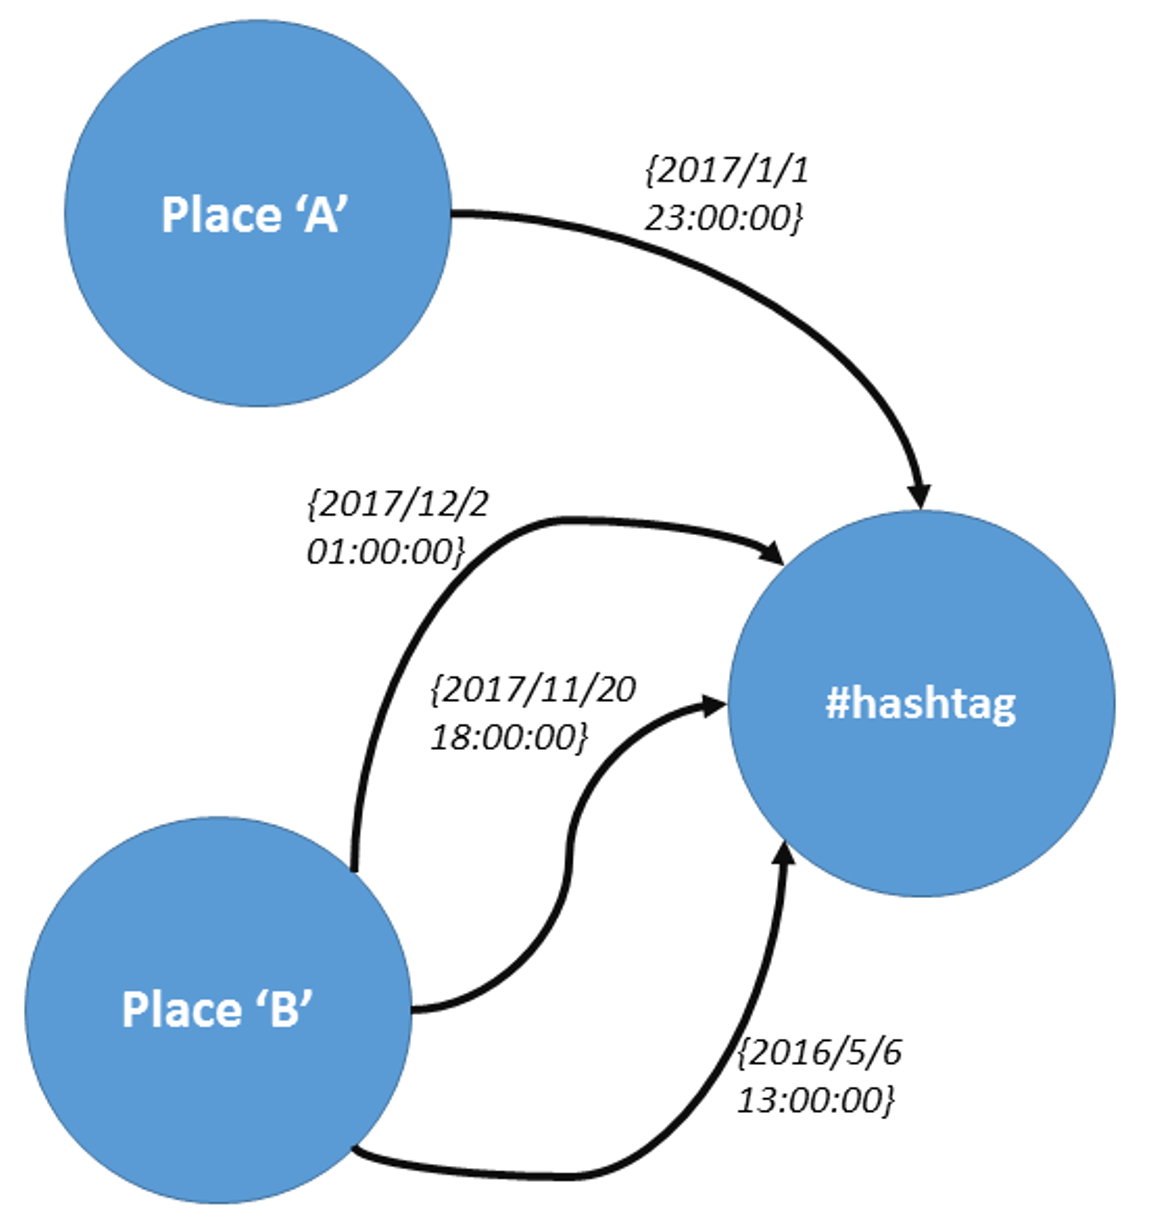
\includegraphics[width=\columnwidth]{images/base_graph.png}
% \caption{Example of weighted base graph}
% \label{fig:basegraph}
% \end{figure}


\subsection{Text analysis and Ngraming}
Trends exist in the form of phrases or hashtags. The main textual 
difference between these is that hashtags appear as a connected 
chain of characters with no whitespaces, while trending phrases include 
spaces. To create a hashtag with more than one word, it must be possible 
to distinguish the words while maintaining their connectivity, and Twitter 
allows underscores to be used in multiple word hashtags. For languages 
such as English, letter capitalisation is an additional popular option in social 
media for hashtaging, such as \#ThisIsAnExample. However, languages 
such as Arabic, Urdu, and Farsi, do not employ capitalisation in the same 
way, therefore the only means of separating words is to use underscores. 
The textual analysis in this study required the trend texts to be tokenized 
to generate ngrams. This process was straightforward for the phrase trends, 
although the hashtag trends included a number of variations that required 
consideration during the textual processing. In capitalized English hashtags, 
for example, it was unclear whether the capital letters referred to the 
beginning of words or abbreviations. In contrast, Arabic hashtags use 
underscores to separate words, which therefore make word separation an 
easy and accurate task to accomplish. As the sample countries were from the 
Arab region, it was anticipated that most tweeting activity would occur in the 
Arabic language, since an earlier study demonstrated that 72\% of all tweets 
in the Arab region are in Arabic [94]. 

In this present study, the textual analysis accounted for underscores and spaces 
only where they occurred as word separators. While this implied that capitalized 
hashtags should be considered as a single word, this would not provide an accurate 
analysis for this group of trends, but since Arabic trends were dominant in the dataset, 
and only capitalized hashtags were affected, this was not anticipated to have an impact 
on the results of the analysis.


\subsection{Derived Graph: Trend-Ngrams}

This directed graph utilized the trend nodes in the base graph to generate its nodes and 
edges. It included two types of nodes: trend and ngram. To generate ngrams from a 
trend, the trend first required tokenization. The trends displayed in two forms, either as 
a phrase, such as 'coffee international day', or a hashtag such as '{\texttt{\#coffee\_international\_day}}'. 
Phrase trends can be tokenized from their original form, while hashtags do not include spaces, 
and hence appear as one word, and therefore first required processing in order that all of the 
trends were translated into phrase form before being tokenized. The hashtags processing 
involved stripping them of the '\#' sign, and replacing the underscores with spaces. Then, 
preserving the word order, the phrases were tokenized, and all possible ngrams then generated. 
The original trend was connected to all of the ngrams generated, and an additional length attribute 
was added to each node within the graph, as shown in lines seven and nine in Algorithm ‎4 4. 
This attribute was used later in the analysis and the visualization setting. Applying this 
algorithm to the hashtag '{\texttt{\#coffee\_international\_day}}' resulted in the graph shown 
in Figure~\ref{fig:tngraph}.

% \begin{figure}[htb] \centering
% 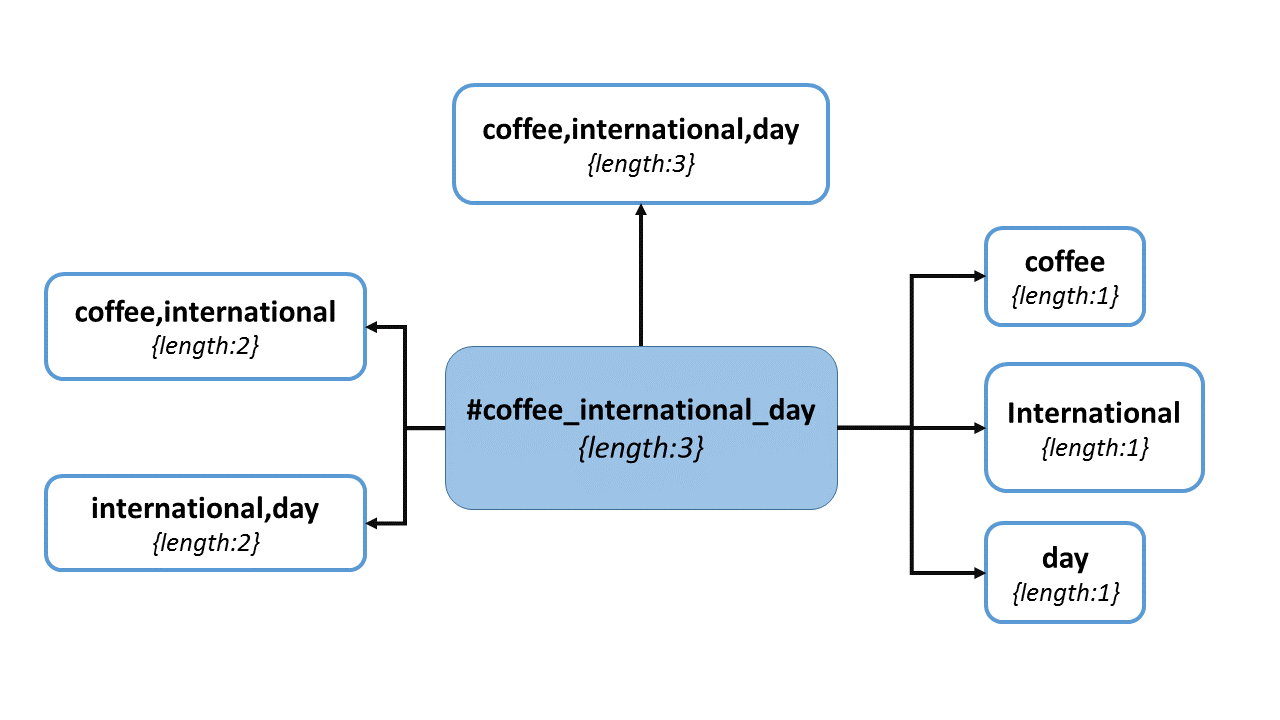
\includegraphics[width=\columnwidth]{images/trend_ngram_example.png}
% \caption{Trend-Ngram graph example}
% \label{fig:tngraph}
% \end{figure}

A trend node in the base graph cannot be repeated. Therefore, the edges linking 
the trend to the ngrams in this graph were expected to have a fixed weight of 1. 
However, observation of the edge weights revealed edges with higher weights, namely 
2 and 3, occurring in trends with repeated words, such as '{\texttt{\#welcome\_you\_welcome}}.
In total, 264 trends had two repeated words, while five trends had three. Since this small number 
of cases fell outside the context of this study, and the analysis of this graph did not utilize individual 
edge weights, they did not affect the results. As a result, only the indegree and outdegree 
centrality measures were employed for this graph, with both the indegree of all of the trend nodes, 
and the outdegree of the ngram nodes being 0. These two measures were employed in the analysis 
phase to distinguish the node types. Furthermore, the indegree of the ngram nodes reflected the 
number of the connected trend, and was at least 1. The outdegree of the trend nodes indicated 
the number of related ngrams. As the ngrams were generated from the trends, the outdegree of 
the trend was found to be fixed, and was equivalent to (n(n+1))/2, where n is length of trend.

\section{Results}\label{results}

Observation of the weighted graph provided an overall evaluation of
activity for trends and places. In total there were 76,266 distinct
trends that trended 2,307,163 times across all locations; this
suggests that trends may appear repeatedly over time. The overall
repetition ratio in the dataset was 97\%, and ranged from 80\% to 98\%
for individual locations, with Saudi Arabia scoring lowest and Qatar
scoring highest rate. {\emph{Indegree}}, {\emph{outdegree}}, and
{\emph{edges}} were used to conduct subsequent results, with further
explanation to follow in the relevant sections.

\subsection{Trend texts: processing and features}
As can be seen in  Figure ~\ref{fig:trends_lengths_wind}, two-word trends 
were the most common trends. Presence of 1 and 3-word trends were at 
similar level, and 4-word trend are a little lower. Then, lengths started to 
show dramatic drop from 5-word onwards. Additionally, weighted indegree 
of trend was found strongly correlated with the word length.

\begin{figure}[htb] \centering
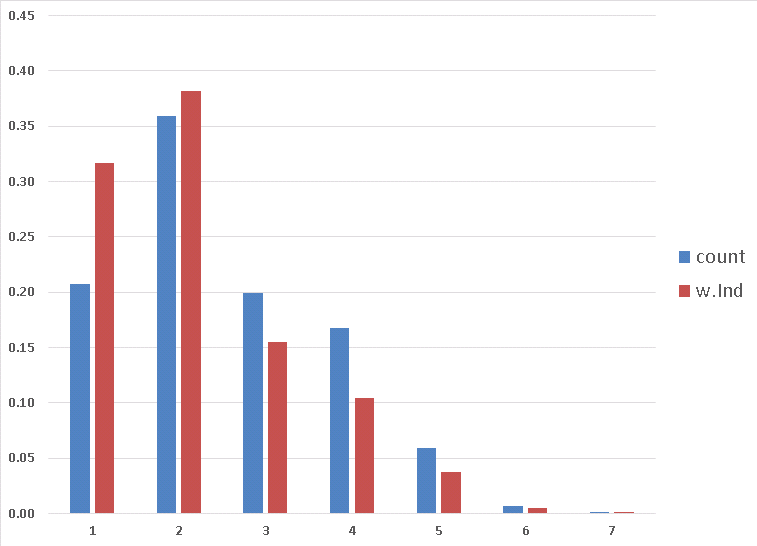
\includegraphics[width=\columnwidth]{images/trends_lengths_wind.png}
\caption{Ratios of trend lengths and their weighted indegree}
\label{fig:tngraph}
\end{figure}

A single odd case was found in which processing the trend’s text resulted 
in 16 words, which indicate very unusual case. Further investigation uncovered 
that the trend consists of three words that were intentionally letter spaced, 
seemingly for fun. To clarify it further, the trend was in Arabic and it is the 
equivalent of {\texttt{\#WriteInSeparateLetters} but was written as 
{\texttt#w_r_i_t_e_I_n_S_e_p_a_r_a_t_e_L_e_t_t_e_r_s. 
Therefore, this was removed from the dataset before progressing to 
further analysis. This demonstrates additional benefit of analysing length 
of trend in removing such odd cases.
\section{Conclusions}\label{conclusions}


%\section*{Acknowledgment}

% BibTeX users
\bibliographystyle{IEEEtran}      % basic style, author-year citations
\bibliography{asonam2018}

\end{document}
